\documentclass[25pt, a0paper, landscape]{tikzposter}
\tikzposterlatexaffectionproofoff
\usepackage[utf8]{inputenc}
\usepackage{authblk}
\makeatletter
\renewcommand\maketitle{\AB@maketitle} % revert \maketitle to its old definition
\renewcommand\AB@affilsepx{\quad\protect\Affilfont} % put affiliations into one line
\makeatother
\renewcommand\Affilfont{\Large} % set font for affiliations
\usepackage{amsmath, amsfonts, amssymb}
\usepackage{tikz}
\usepackage{pgfplots}
% align columns of tikzposter; needs two compilations
\usepackage[colalign]{column_aligned}

% tikzposter meta settings
\usetheme{Default}
\usetitlestyle{Default}
\useblockstyle{Default}

%%%%%%%%%%% redefine title matter to include one logo on each side of the title; adjust with \LogoSep
\makeatletter
\newcommand\insertlogoi[2][]{\def\@insertlogoi{\includegraphics[#1]{#2}}}
\newcommand\insertlogoii[2][]{\def\@insertlogoii{\includegraphics[#1]{#2}}}
\newlength\LogoSep
\setlength\LogoSep{-70pt}

\renewcommand\maketitle[1][]{  % #1 keys
    \normalsize
    \setkeys{title}{#1}
    % Title dummy to get title height
    \node[inner sep=\TP@titleinnersep, line width=\TP@titlelinewidth, anchor=north, minimum width=\TP@visibletextwidth-2\TP@titleinnersep]
    (TP@title) at ($(0, 0.5\textheight-\TP@titletotopverticalspace)$) {\parbox{\TP@titlewidth-2\TP@titleinnersep}{\TP@maketitle}};
    \draw let \p1 = ($(TP@title.north)-(TP@title.south)$) in node {
        \setlength{\TP@titleheight}{\y1}
        \setlength{\titleheight}{\y1}
        \global\TP@titleheight=\TP@titleheight
        \global\titleheight=\titleheight
    };

    % Compute title position
    \setlength{\titleposleft}{-0.5\titlewidth}
    \setlength{\titleposright}{\titleposleft+\titlewidth}
    \setlength{\titlepostop}{0.5\textheight-\TP@titletotopverticalspace}
    \setlength{\titleposbottom}{\titlepostop-\titleheight}

    % Title style (background)
    \TP@titlestyle

    % Title node
    \node[inner sep=\TP@titleinnersep, line width=\TP@titlelinewidth, anchor=north, minimum width=\TP@visibletextwidth-2\TP@titleinnersep]
    at (0,0.5\textheight-\TP@titletotopverticalspace)
    (title)
    {\parbox{\TP@titlewidth-2\TP@titleinnersep}{\TP@maketitle}};

    \node[inner sep=0pt,anchor=west] 
    at ([xshift=-\LogoSep]title.west)
    {\@insertlogoi};

    \node[inner sep=0pt,anchor=east] 
    at ([xshift=\LogoSep]title.east)
    {\@insertlogoii};

    % Settings for blocks
    \normalsize
    \setlength{\TP@blocktop}{\titleposbottom-\TP@titletoblockverticalspace}
}
\makeatother
%%%%%%%%%%%%%%%%%%%%%%%%%%%%%%%%%%%%%


% color handling
\definecolor{TumBlue}{cmyk}{1,0.43,0,0}
\colorlet{blocktitlebgcolor}{TumBlue}
\colorlet{backgroundcolor}{white}

% title matter
\title{Disease Type Prediction}
\author[1]{Zhen Yan}
\author[1]{Yumin Sun}
\author[1]{Yuchang Zhang}
\author[1]{Xiaojing Li}

\affil[1]{Technical University of Munich}

\insertlogoi[width=15cm]{tum_logo}
\insertlogoii[width=15cm]{tum_logo}

% main document
\begin{document}

\maketitle

\begin{columns}
    \column{0.3}
    \block{Abstract}{Chest X-ray is a widely used medical imaging procedures. A large hospital typically produces over 40,000 chest X-rays per year. However, lacking qualified radiologists to review these X-rays is a major challenge. Reviewing chest X-rays heavily depends on the experience of radiologists and many images are difficult to read when the lesions are in low contrast or overlap with large pulmonary vessels. Since CNN shows an ability to extract hight level features, we explore the possibility of designing computer aided diagnosis for chest X-rays using deep learning approach. We work on 18,000+ images provided from Hackerearth Deep Learning Challenge Cup(HDLCC) to predict single-disease. At last we reach 0.41 weighted f1 score on final off-line test set, with which we locate in the 20th place in the HDLCC (rank 20 / 151 solved / 7079 participants).}    
    \block{Data pre-processing and augmentation}{
    \textbullet \textbf{Datasets}\newline
    The dataset includes 18,000+ chest X-ray images of size 1024*1024*1. There are in total 14 diseases and the dataset is strongly unbalanced with 5000+ images from most likely diseases and 50+ images from most unlikely diseases.\\
    \textbullet \textbf{Pre-processing and augmentation}\newline
    Due to the low contrast in details in X-ray images, image pre-processing is an essential step to gain features. We first improve contrast using equalized histogram and then saturate the darkest and lightest of 0.5\% gray values. We also did data augmentation to avoid over-fitting. And we find out even rotation and flips also help to avoid over-fitting, though intuitively those augmented images could never happen in nature.
    
    \begin{center}
    	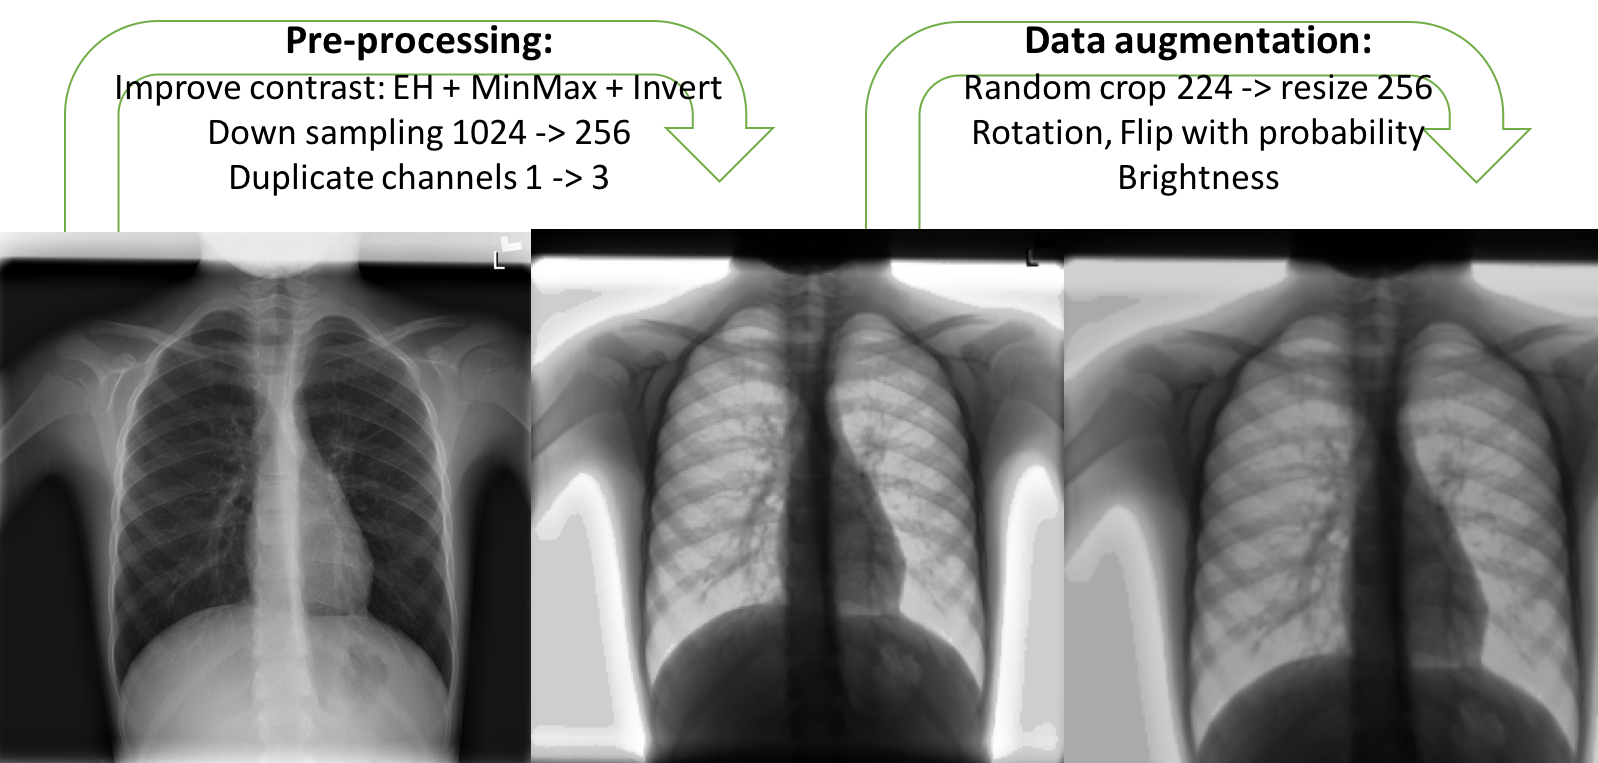
\includegraphics[scale=1]{aug_poster.png}
    \end{center}
    
    
    
    
    }
    
 
    \column{0.45}
    \block{Architecture}{
    \textbullet \textbf{Scalable random weighted sampler}\newline
    We designed scalable weighted sample to balance the difference of numbers of different types of dieseases.  $$y=\alpha x_{i}^\beta, \ \alpha = \sqrt{{\max({x_{i}})}}$$
    where 
    $x_{i}$ is original number of images of $i^{th}$ disearse, $\beta \in [0.5, 1.2]$ is paramter, $y_{i}$ is number of images of $i$th disearse after weighted.\\
    \begin{center}
    	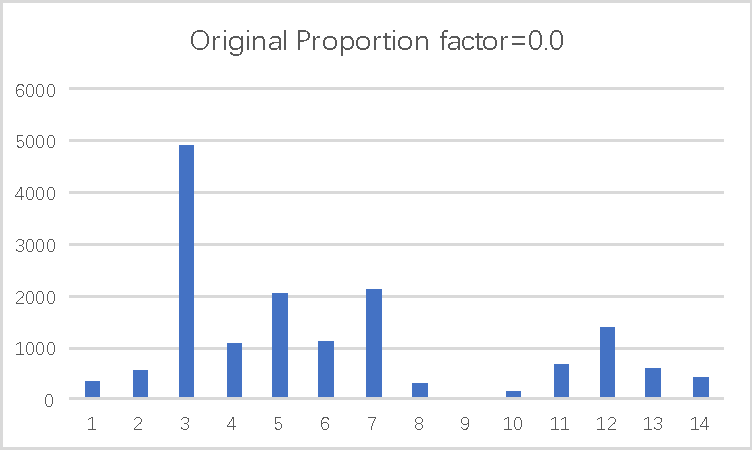
\includegraphics[scale=0.9]{assets/factor_0_0.pdf}
        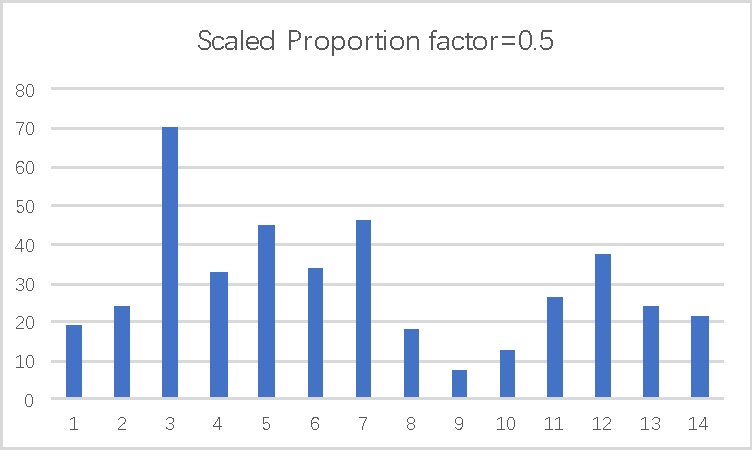
\includegraphics[scale=0.9]{assets/factor_0_5.pdf}
        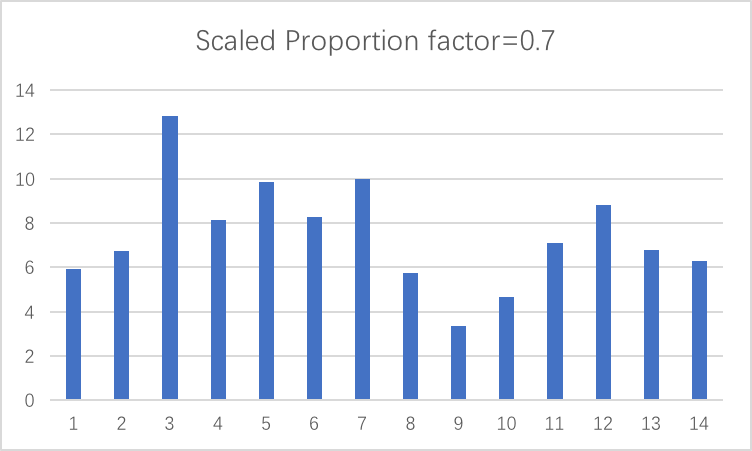
\includegraphics[scale=0.9]{assets/factor_0_7.png}
        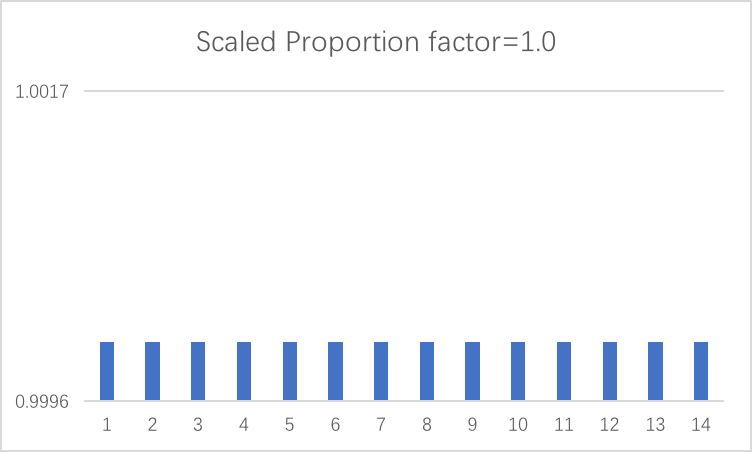
\includegraphics[scale=0.9]{assets/factor_1_0.png}
    \end{center}
    \textbullet \textbf{Learning-rate scheduler}\newline
    Learning rate scheduler is used to accelerate the convergence speed of neural network.\newline
    \textbullet \textbf{Bayesian optimization}\newline
    Optimatize a blackbox, where we input the range of paramters and try to reach better accuacy with the respective paramters.
    $$x^*= arg \max a_{LCB}(x; {x_n, y_n}, \theta)$$
    where $$a_{LCB}(x; {x_n, y_n}, \theta)= \mu ( x; { x_n, y_n}, \theta)- \kappa \sigma(x; {x_n, y_n}, \theta)$$
    \begin{center}
    	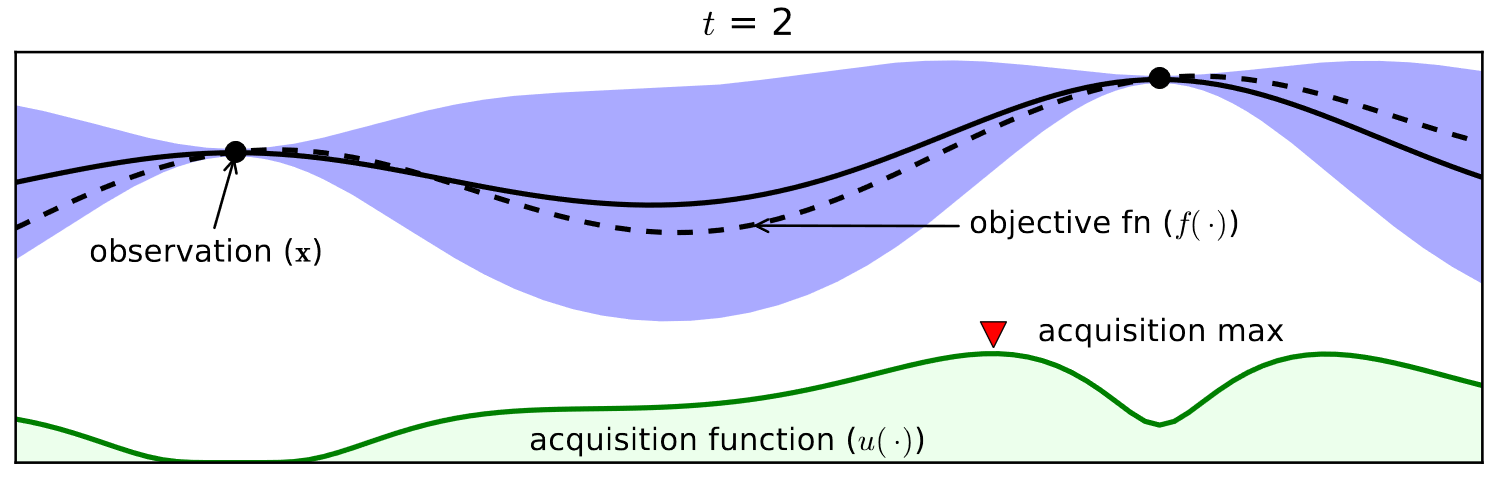
\includegraphics[scale=0.3]{assets/bo1.png}
        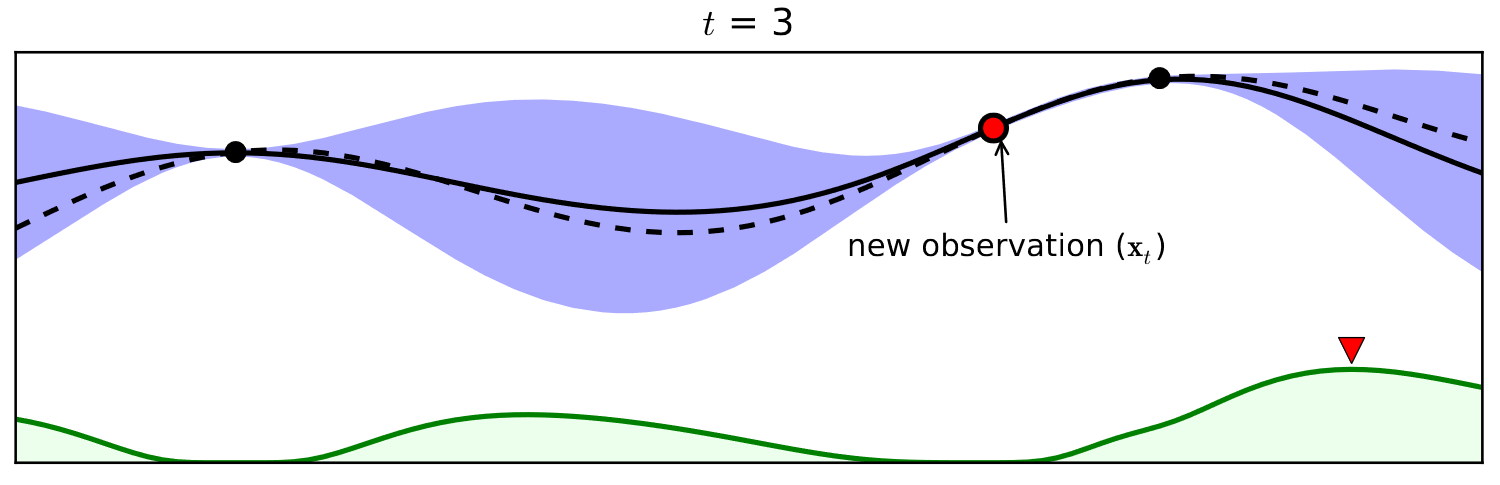
\includegraphics[scale=0.3]{assets/bo2.png}
        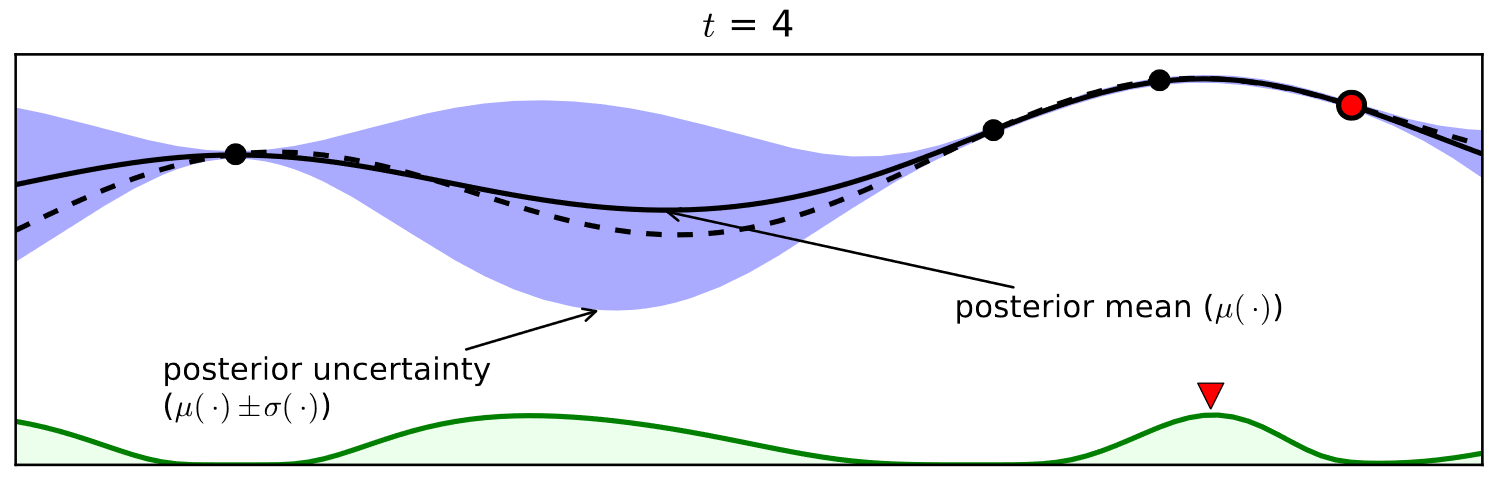
\includegraphics[scale=0.3]{assets/bo3.png}
    \end{center}
    \textbullet \textbf{Network}\newline
    We treat the denset$121$ network as the blackbox.
    \begin{center}
    	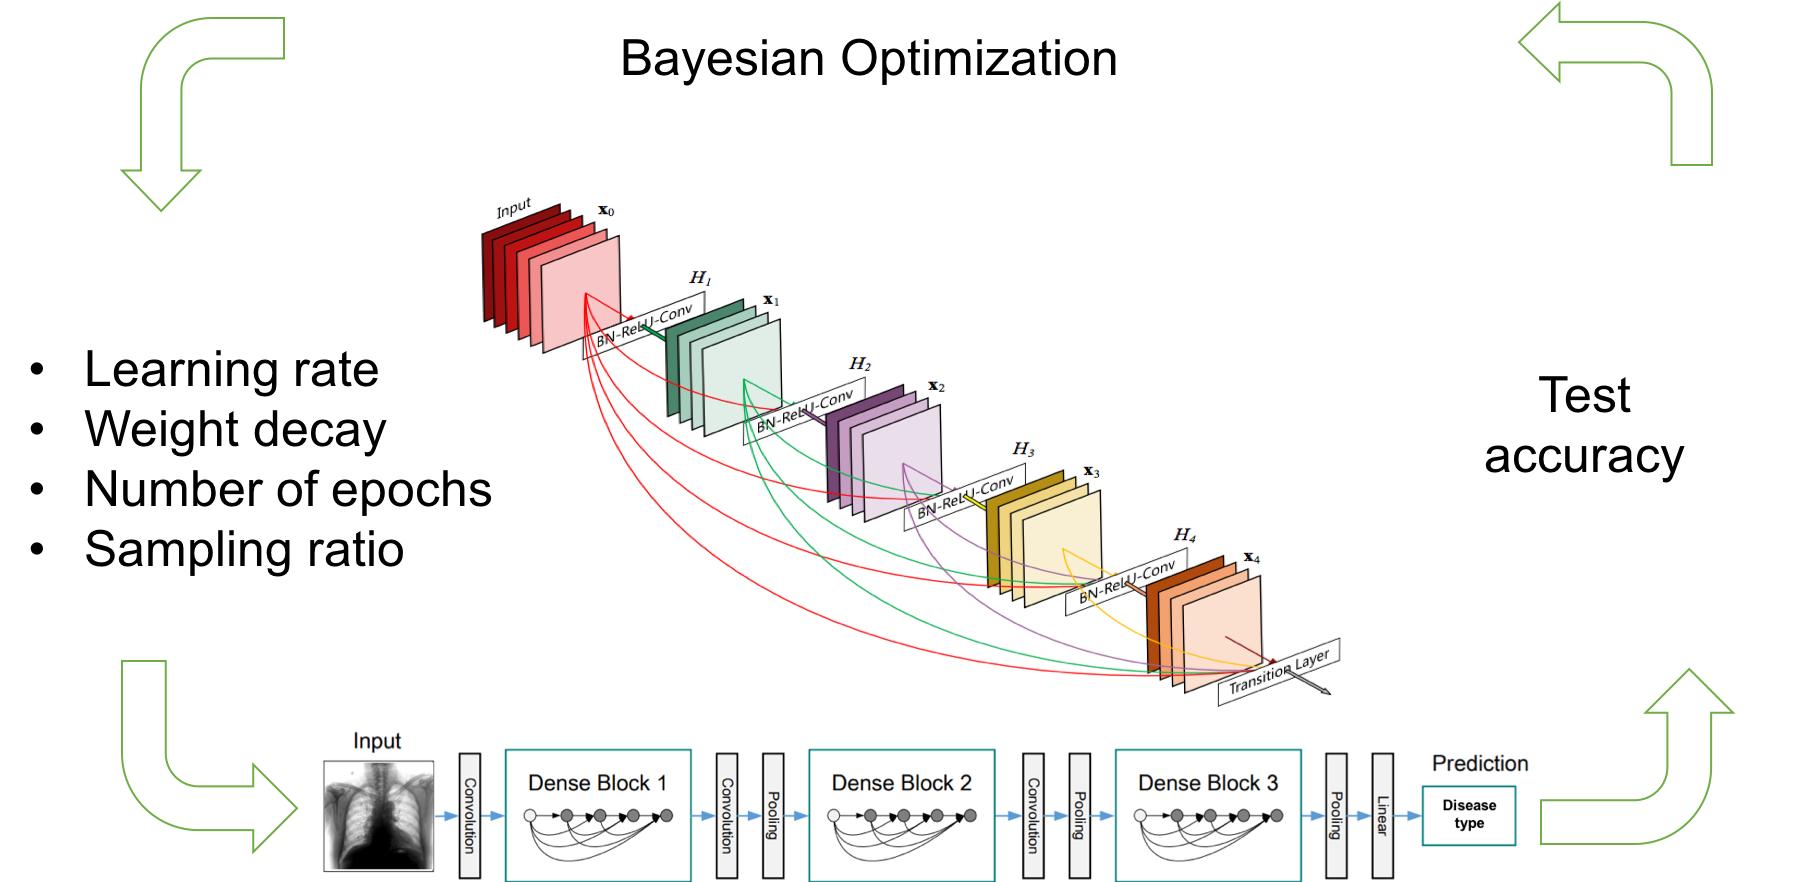
\includegraphics[scale=1.5]{bayesOpt.png}
    \end{center}
    }
    
    \column{0.25}
    \block{Results}{
     \textbullet\textbf{Our Position}\newline
   $~~~$---F$1$ Score
    $$F_1 = 2 \cdot \frac{precision \cdot recall}{precision + recall}$$
    \begin{center}
    	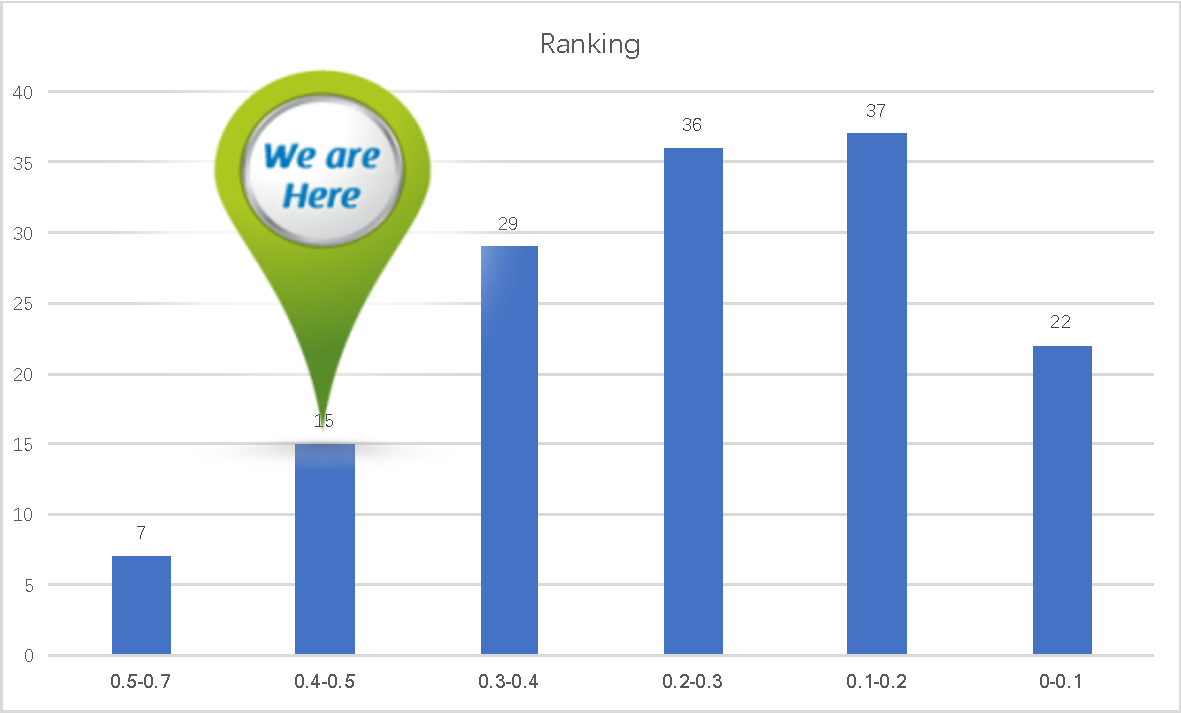
\includegraphics[scale=0.95]{assets/here.pdf}
    \end{center}
    
     \textbullet\textbf{Solved/Unsolved Ratio}\newline
    \begin{center}
    	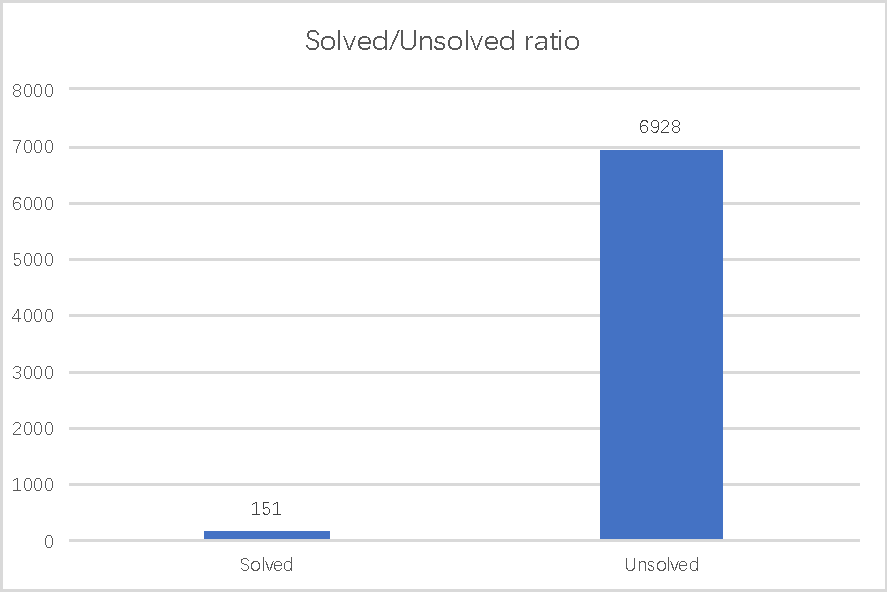
\includegraphics[scale=1.3]{assets/ratio.pdf}
    \end{center}
    
    
    
    
    
    
    
    }
    \block{Conclusion}{In this project, 18000+ X-ray images of total 14 diseases are trained on alexnet, vgg16, desnet121 and resnet18-101. It shows that they all produced similar results with variance of depth and models. However, training on the pre-trained feature extraction layers usually yields better results than freezing these layers. We therefore conclude that X-ray images indeed have different structures than nature images, so that the general used CNNs are not able to transfered directly to medical images. Considering the highly unbalanced dataset, scalable random weighted sampler and data augmentation are applied. To accelerate the training process, learning rate scheduler and bayesian optimization are introduced. Due to limited image quantity, we could not reach a considerable high accuracy and the final result reaches weighted F1 score of 0.41.
    
    
    
    
    
    
    }
\end{columns}

\end{document}
